%!TEX TS-program = pdflatex
%!TEX TS-options = -shell-escape
% ============================================================
%  Einführung in die Programmiersprache Rust
%  Vorlesung Embedded Systems Engineering
%  Prof. Dr.-Ing. Sebastian Schlesinger
%  HWR Berlin, Wintersemester 2026
% ============================================================

% xcolor muss vor beamer mit Optionen gepatcht werden
\PassOptionsToPackage{usenames,x11names}{xcolor}

\documentclass[%
  aspectratio=169,
  10pt
]{beamer}

% -----------------------------------------------------------
%  Sprache und Encoding
% -----------------------------------------------------------
\usepackage[utf8]{inputenc}
\usepackage[T1]{fontenc}
% Deutsche Anführungszeichen (ohne babel-german)
\usepackage{textcomp}
\newcommand{\enquote}[1]{\quotedblbase{}#1\textquotedblleft{}}

% -----------------------------------------------------------
%  Fonts
% -----------------------------------------------------------
\usepackage{charter}
\usepackage{courier}                % Monospace-Font für Listings
\renewcommand{\ttdefault}{pcr}      % Courier als tt-Font
% microtype: nur protrusion, kein font-expansion (Beamer-kompatibel)
\usepackage[protrusion=true,expansion=false]{microtype}

% -----------------------------------------------------------
%  Farben  (wie config.tex der Übungsblätter)
% -----------------------------------------------------------
\definecolor{fbblau}{HTML}{3078AB}
\definecolor{blackberry}{rgb}{0.53, 0.0, 0.25}
\definecolor{codebg}{rgb}{0.97, 0.97, 0.97}
\definecolor{rustcolor}{HTML}{CE422B}

% -----------------------------------------------------------
%  Beamer-Theme (angepasst an ESE-Stil)
% -----------------------------------------------------------
\usetheme{default}
\useinnertheme{rectangles}

%  Strukturfarbe
\setbeamercolor{structure}{fg=fbblau}

%  Titelfolie
\setbeamercolor{title}{fg=white, bg=fbblau}
\setbeamercolor{subtitle}{fg=fbblau!25!white, bg=fbblau}
\setbeamercolor{author}{fg=white, bg=fbblau}
\setbeamercolor{institute}{fg=fbblau!20!white, bg=fbblau}
\setbeamercolor{date}{fg=fbblau!20!white, bg=fbblau}

%  Folienrahmen
\setbeamercolor{frametitle}{fg=white, bg=fbblau}
\setbeamerfont{frametitle}{series=\bfseries, size=\normalsize}

%  Inhaltsverzeichnis
\setbeamercolor{section in toc}{fg=fbblau}
\setbeamerfont{section in toc}{series=\bfseries}

%  Blöcke
\setbeamercolor{block title}{bg=fbblau, fg=white}
\setbeamercolor{block body}{bg=fbblau!8, fg=black}
\setbeamercolor{alertblock title}{bg=blackberry, fg=white}
\setbeamercolor{alertblock body}{bg=blackberry!8, fg=black}
\setbeamercolor{exampleblock title}{bg=fbblau!70!black, fg=white}
\setbeamercolor{exampleblock body}{bg=fbblau!6, fg=black}

%  Aufzählungspunkte
\setbeamercolor{item}{fg=fbblau}
\setbeamercolor{subitem}{fg=fbblau!70}
\setbeamertemplate{itemize item}{\small$\triangleright$}
\setbeamertemplate{itemize subitem}{\small$\triangleright$}

%  Navigationsleiste ausblenden
\setbeamertemplate{navigation symbols}{}

%  Fußzeile
\setbeamertemplate{footline}{%
  \leavevmode
  \hbox{%
    \begin{beamercolorbox}[wd=.50\paperwidth,ht=2.25ex,dp=1ex,
                           left,leftskip=2mm]{palette primary}%
      \usebeamerfont{author in head/foot}%
      \textbf{ESE} \,|\, Einführung in Rust \,|\, \insertshortauthor
    \end{beamercolorbox}%
    \begin{beamercolorbox}[wd=.40\paperwidth,ht=2.25ex,dp=1ex,
                           center]{palette secondary}%
      \usebeamerfont{title in head/foot}\insertsection
    \end{beamercolorbox}%
    \begin{beamercolorbox}[wd=.10\paperwidth,ht=2.25ex,dp=1ex,
                           right,rightskip=2mm]{palette primary}%
      \insertframenumber\,/\,\inserttotalframenumber
    \end{beamercolorbox}%
  }%
}

%  Sectiontrenner
\AtBeginSection[]{%
  \begin{frame}[plain]
    \vfill
    \centering
    \begin{beamercolorbox}[sep=12pt,center,shadow=false,rounded=false,
                           wd=0.8\textwidth]{title}
      \usebeamerfont{title}\insertsectionhead
    \end{beamercolorbox}
    \vfill
  \end{frame}
}

% -----------------------------------------------------------
%  Code-Listings  (Rust-Konfiguration)
% -----------------------------------------------------------
\usepackage{listings}

% Rust-Sprachdefinition für listings
\lstdefinelanguage{Rust}{%
  keywords=[1]{fn, let, mut, const, static, if, else, match, loop, while,
               for, in, break, continue, return, struct, enum, impl, trait,
               type, where, as, use, mod, pub, crate, self, Self, super,
               move, ref, unsafe, extern, async, await, dyn, box, yield},
  keywords=[2]{i8, i16, i32, i64, i128, isize,
               u8, u16, u32, u64, u128, usize,
               f32, f64, bool, char, str, String,
               Vec, Option, Result, Some, None, Ok, Err,
               Box, Rc, Arc, Cell, RefCell, Mutex,
               true, false, println, print, format, vec,
               Copy, Clone, Debug, Display, Default, PartialEq, Eq,
               PartialOrd, Ord, Hash, Send, Sync, Sized, Drop, Fn, FnMut, FnOnce,
               Iterator, IntoIterator, From, Into, TryFrom, TryInto},
  keywords=[3]{derive, cfg, test, allow, deny, warn, inline, no_mangle,
               repr, no_std, global_allocator, panic_handler, entry},
  sensitive=true,
  morecomment=[l]{//},
  morecomment=[s]{/*}{*/},
  morestring=[b]",
  morestring=[b]',
}

\lstset{%
  language        = Rust,
  basicstyle      = \ttfamily\scriptsize,
  keywordstyle    = [1]\color{fbblau}\bfseries,
  keywordstyle    = [2]\color{blackberry},
  keywordstyle    = [3]\color{fbblau!70!black}\itshape,
  commentstyle    = \color{gray}\itshape,
  stringstyle     = \color{blackberry},
  numberstyle     = \tiny\color{gray},
  numbers         = left,
  numbersep       = 6pt,
  stepnumber      = 1,
  frame           = single,
  framesep        = 2pt,
  rulecolor       = \color{fbblau!40},
  backgroundcolor = \color{codebg},
  showstringspaces= false,
  breaklines      = true,
  columns         = fullflexible,
  keepspaces      = true,
  xleftmargin     = 1.0em,
  xrightmargin    = 0.2em,
  tabsize         = 4,
  aboveskip       = 4pt,
  belowskip       = 2pt,
  % Umlaute in lstlisting-Umgebungen ermöglichen
  literate        = {ä}{{\"a}}1 {ö}{{\"o}}1 {ü}{{\"u}}1
                    {Ä}{{\"A}}1 {Ö}{{\"O}}1 {Ü}{{\"U}}1
                    {ß}{{\ss}}1
}

% -----------------------------------------------------------
%  Weitere Pakete
% -----------------------------------------------------------
\usepackage{tikz}
\usetikzlibrary{arrows.meta, shapes, positioning, calc, matrix, fit}
\usepackage{booktabs}
\usepackage{array}
\usepackage{multicol}

% -----------------------------------------------------------
%  Metadaten
% -----------------------------------------------------------
\title[Einführung in Rust]{Einführung in die Programmiersprache Rust}
\subtitle{Embedded Systems Engineering -- Vorlesung}
\author[Schlesinger]{Prof.\,Dr.\,-Ing.\ Sebastian Schlesinger}
\institute{%
  Fachbereich 2 -- Duales Studium Wirtschaft \& Technik\\
  HWR Berlin}
\date{Wintersemester 2026}

% ============================================================
\begin{document}
% ============================================================

% -----------------------------------------------------------
%  TITELFOLIE
% -----------------------------------------------------------
\begin{frame}[plain]
  \titlepage
\end{frame}

% -----------------------------------------------------------
%  GLIEDERUNG
% -----------------------------------------------------------
\begin{frame}{Gliederung}
  \tableofcontents
\end{frame}

% ============================================================
\section{Motivation und Geschichte}
% ============================================================

\begin{frame}{Warum Rust? -- Die Probleme von C}
  \begin{columns}[T]
    \begin{column}{0.48\textwidth}
      \small
      \textbf{Bekannte C-Schwächen:}
      \begin{itemize}
        \item \textbf{Speicherfehler:} Buffer Overflows, Use-after-Free,
              Dangling Pointer, Double Free
        \item \textbf{Undefined Behavior:} stille Korrumpierung
              statt kontrolliertem Fehler
        \item \textbf{Kein Modulsystem:} nur \texttt{\#include}
              und Linker
        \item \textbf{Kein echtes Typsystem} für Generizität --
              nur \texttt{void*} mit Casts
        \item \textbf{Manuelle Ressourcenverwaltung:}
              vergessenes \texttt{free()}, Memory Leaks
      \end{itemize}
    \end{column}
    \begin{column}{0.48\textwidth}
      \small
      \textbf{Was Rust verspricht:}
      \begin{itemize}
        \item \textbf{Memory Safety ohne GC} --
              zur Compile-Zeit garantiert
        \item \textbf{Zero-Cost Abstractions:} Generics,
              Iteratoren, Pattern Matching -- ohne Overhead
        \item \textbf{Data Race Freedom:} Compiler verhindert
              gleichzeitige mutable Zugriffe
        \item \textbf{Modernes Tooling:} Cargo (Build + Deps),
              Clippy (Linter), Rustfmt
        \item \textbf{C-äquivalente Performance:}
              kein Runtime, kein GC, LLVM-Backend
      \end{itemize}
    \end{column}
  \end{columns}
  \vspace{0.3em}
  \begin{alertblock}{Leitsatz}
    \emph{Rust bietet die Kontrolle von C -- mit den Sicherheitsgarantien moderner Sprachen.}
  \end{alertblock}
\end{frame}

\begin{frame}{Geschichte und Ökosystem}
  \begin{columns}[T]
    \begin{column}{0.58\textwidth}
      \small
      \textbf{Entwicklungsgeschichte:}
      \begin{itemize}
        \item \textbf{2006} -- Graydon Hoare startet Rust als
              persönliches Projekt bei Mozilla
        \item \textbf{2009} -- Mozilla sponsert offiziell die Entwicklung
        \item \textbf{2015} -- \textbf{Rust 1.0} -- erste stabile Version,
              Stabilität durch \emph{Editions}-System
        \item \textbf{2021} -- Gründung der \textbf{Rust Foundation}
              (AWS, Google, Huawei, Microsoft, Mozilla)
        \item \textbf{2022} -- Linux-Kernel akzeptiert Rust als
              \emph{zweite Sprache} neben C
        \item \textbf{2024+} -- Rust in Android, Windows-Kernel,
              Chromium, kritischer Infrastruktur
      \end{itemize}
    \end{column}
    \begin{column}{0.38\textwidth}
      \small
      \begin{block}{Editions (Kompatibilität)}
        \textbf{2015} -- Erstausgabe\\
        \textbf{2018} -- async/await, Module\\
        \textbf{2021} -- Closures, Patterns\\
        \textbf{2024} -- neueste Edition\\[0.2em]
        Verschiedene Editions sind \emph{innerhalb}
        eines Projekts mischbar!
      \end{block}
      \begin{exampleblock}{Toolchain}
        \texttt{rustup} -- Installer/Updater\\
        \texttt{cargo} -- Build + Paketmanager\\
        \texttt{rustc} -- Compiler (LLVM)\\
        \texttt{clippy} -- Linter\\
        \texttt{rustfmt} -- Autoformatter
      \end{exampleblock}
    \end{column}
  \end{columns}
  \vspace{0.2em}
  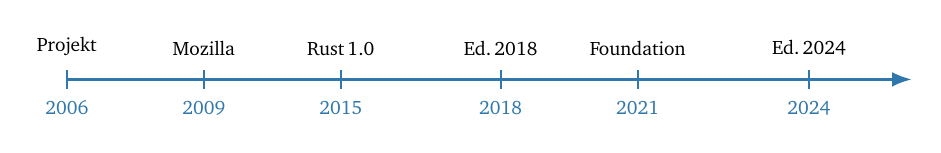
\begin{tikzpicture}[x=1.45cm]
    \draw[-{Latex[length=2.5mm]}, thick, fbblau] (0,0) -- (7.4,0);
    \foreach \pos/\lab/\desc in {%
      0/{2006}/{Projekt},
      1.2/{2009}/{Mozilla},
      2.4/{2015}/{Rust\,1.0},
      3.8/{2018}/{Ed.\,2018},
      5/{2021}/{Foundation},
      6.5/{2024}/{Ed.\,2024}}{%
      \draw[fbblau, thick] (\pos, 0.12) -- (\pos, -0.12);
      \node[below, fbblau, font=\scriptsize] at (\pos, -0.15) {\lab};
      \node[above, font=\scriptsize]         at (\pos,  0.18) {\desc};
    }
  \end{tikzpicture}
\end{frame}

\begin{frame}[fragile]{Vergleich: Hello World in C und Rust}
  \begin{columns}[T]
    \begin{column}{0.46\textwidth}
      \textbf{C:}
\begin{lstlisting}[language=C,morekeywords={printf}]
#include <stdio.h>

int main(void) {
    printf("Hello, ESE!\n");
    return 0;
}
\end{lstlisting}
      \textbf{Kompilierung:}\\
      {\small\texttt{gcc -std=c11 -Wall -o hello hello.c}\\
      \texttt{./hello}}
    \end{column}
    \begin{column}{0.50\textwidth}
      \textbf{Rust:}
\begin{lstlisting}
fn main() {
    println!("Hello, ESE!");
}
\end{lstlisting}
      \textbf{Kompilierung:}\\
      {\small\texttt{cargo new hello \&\& cd hello}\\
      \texttt{cargo run}}
      \vspace{0.3em}
      \begin{block}{Was fällt auf?}
        \small
        \begin{itemize}
          \item Kein \texttt{\#include} -- Modulsystem mit \texttt{use}
          \item \texttt{println!} ist ein \emph{Makro} (\texttt{!})
          \item Kein explizites \texttt{return 0} nötig
          \item Cargo erzeugt Projektstruktur automatisch
        \end{itemize}
      \end{block}
    \end{column}
  \end{columns}
\end{frame}

% ============================================================
\section{Typsystem und Grundkonstrukte}
% ============================================================

\begin{frame}[fragile]{Variablen, Mutabilität und Typen}
  \begin{columns}[T]
    \begin{column}{0.48\textwidth}
      \textbf{Variablen und Bindungen:}
\begin{lstlisting}
// Immutable per Default!
let x = 42;
// x = 43;  // Fehler!

// Explizit mutable
let mut counter = 0;
counter += 1;  // OK

// Shadowing (Neubindung)
let x = x + 1;        // OK: neues x
let x = "jetzt Text";  // anderer Typ!

// Konstanten (zur Compilezeit)
const MAX_SIZE: usize = 128;
\end{lstlisting}
    \end{column}
    \begin{column}{0.48\textwidth}
      \textbf{Skalare Typen:}
      \begin{block}{}
        \scriptsize
        \begin{tabular}{l l l}
          \texttt{i8..i128}  & vorzeichenbeh. & fest\\
          \texttt{u8..u128}  & vorzeichenlos  & fest\\
          \texttt{isize/usize} & ptr-breit    & arch.\\
          \texttt{f32, f64}  & Gleitkomma     &\\
          \texttt{bool}      & \texttt{true}/\texttt{false} &\\
          \texttt{char}      & 4 Byte Unicode &
        \end{tabular}
      \end{block}
      \textbf{Zusammengesetzte Typen:}
\begin{lstlisting}
// Tupel (heterogen, feste Länge)
let t: (i32, f64, bool) = (42, 3.14, true);
let x = t.0;  // 42

// Array (homogen, feste Länge)
let arr: [u8; 4] = [0xFF; 4];

// Slice (dynamisches Fenster)
let slice: &[u8] = &arr[1..3];
\end{lstlisting}
    \end{column}
  \end{columns}
\end{frame}

\begin{frame}[fragile]{Kontrollstrukturen und Ausdrücke}
  \begin{columns}[T]
    \begin{column}{0.47\textwidth}
      \textbf{if ist ein Ausdruck:}
\begin{lstlisting}
let voltage = 3.3;
let status = if voltage > 3.0 {
    "OK"
} else if voltage > 2.0 {
    "Warnung"
} else {
    "Kritisch"
};  // Ergebnis direkt zuweisbar
\end{lstlisting}
      \textbf{Schleifen:}
\begin{lstlisting}
for i in 0..10 { println!("{}", i); }

while !uart_ready() { /* warten */ }

// loop mit break-Wert
let result = loop {
    let v = adc_read();
    if v > THRESHOLD { break v; }
};
\end{lstlisting}
    \end{column}
    \begin{column}{0.50\textwidth}
      \textbf{Blöcke als Ausdrücke:}
\begin{lstlisting}
// Letzter Ausdruck ohne ; = Rückgabewert
let y = {
    let a = 5;
    let b = 10;
    a + b   // = 15, Wert von y
};
\end{lstlisting}
      \begin{block}{Paradigmenwechsel gegenüber C}
        \small
        \begin{itemize}
          \item C: Anweisungen dominieren;
                Rust: \emph{fast alles} ist ein Ausdruck
          \item \texttt{if}, Blöcke, \texttt{match},
                \texttt{loop} -- alle liefern Werte
          \item Kein ternärer Operator nötig --
                \texttt{if} ersetzt \texttt{?:}
          \item Kein impliziter Fallthrough wie bei C-\texttt{switch}
        \end{itemize}
      \end{block}
    \end{column}
  \end{columns}
\end{frame}

\begin{frame}[fragile]{Funktionen und Typinferenz}
  \begin{columns}[T]
    \begin{column}{0.50\textwidth}
\begin{lstlisting}
// Funktionssignatur: Typen explizit
fn clamp(val: i32, lo: i32, hi: i32) -> i32 {
    if val < lo { lo }
    else if val > hi { hi }
    else { val }  // letzter Ausdruck = return
}

// Unit-Rückgabetyp (wie void in C)
fn greet(name: &str) {
    println!("Hallo, {}!", name);
}

// Frühes return ist möglich
fn divide(a: f64, b: f64) -> Option<f64> {
    if b == 0.0 { return None; }
    Some(a / b)
}

// Generische Funktion
fn max_of<T: PartialOrd>(a: T, b: T) -> T {
    if a >= b { a } else { b }
}
\end{lstlisting}
    \end{column}
    \begin{column}{0.47\textwidth}
      \textbf{Typinferenz:}
\begin{lstlisting}
let x = 42;        // i32 (Default)
let y = 3.14;      // f64 (Default)
let z = x as f64 + y;  // f64

// Turbofish bei Mehrdeutigkeit
let v = "42".parse::<i32>().unwrap();

// Typaliase
type Volt = f32;
type Register = u32;
let reg: Register = 0x4001_0800;
\end{lstlisting}
      \begin{block}{Vergleich zu C}
        \small
        \begin{itemize}
          \item C: alle Typen explizit, keine Inferenz
          \item Rust: lokale Inferenz, aber
                Funktionssignaturen \emph{immer} explizit
          \item Sicherer: kein impliziter
                Integer-Overflow (panic im Debug)
        \end{itemize}
      \end{block}
    \end{column}
  \end{columns}
\end{frame}

% ============================================================
\section{Ownership, Borrowing und Lifetimes}
% ============================================================

\begin{frame}[fragile]{Das Ownership-Prinzip}
  \begin{columns}[T]
    \begin{column}{0.50\textwidth}
      \small
      \textbf{Die drei Regeln:}
      \begin{enumerate}
        \item Jeder Wert hat genau \textbf{einen Owner}
        \item Wird der Owner ungültig (\emph{out of scope}),
              wird der Wert \textbf{automatisch freigegeben}
        \item Ownership kann \textbf{transferiert} werden (\emph{Move})
      \end{enumerate}
\begin{lstlisting}
fn main() {
    let s1 = String::from("Hallo");
    let s2 = s1;  // MOVE: s1 ungültig!
    // println!("{}", s1); // Fehler!
    println!("{}", s2);    // OK
}  // s2 wird hier gedroppt -> Speicher frei
\end{lstlisting}
      \begin{alertblock}{Kein free() nötig!}
        \small Der Compiler fügt \texttt{drop()} automatisch
        am Scope-Ende ein -- keine Leaks, kein
        Double Free, kein Use-after-Free.
      \end{alertblock}
    \end{column}
    \begin{column}{0.47\textwidth}
      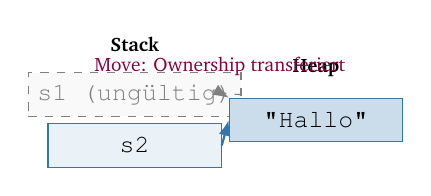
\begin{tikzpicture}[scale=0.72, every node/.style={font=\small}]
        \tikzset{
          membox/.style={draw=fbblau, fill=fbblau!10,
                 minimum width=2.2cm, minimum height=0.55cm,
                 font=\small\ttfamily},
          inv/.style={draw=gray, dashed, fill=gray!5,
                 minimum width=2.2cm, minimum height=0.55cm,
                 font=\small\ttfamily, text=gray}
        }
        \node[inv]    (s1) at (0, 2.2) {s1 (ungültig)};
        \node[membox] (s2) at (0, 1.3) {s2};
        \node[membox, fill=fbblau!25] (heap) at (3.2, 1.75) {"Hallo"};
        \draw[-{Latex[length=2mm]}, thick, fbblau]
          (s2.east) -- (heap.west);
        \draw[-{Latex[length=2mm]}, dashed, gray]
          (s1.east) to[out=0,in=150] (heap.north west);
        \node[above=4pt of s1, font=\bfseries\scriptsize] {Stack};
        \node[above=4pt of heap, font=\bfseries\scriptsize] {Heap};
        \node[font=\scriptsize, blackberry] at (1.5, 2.7) {Move: Ownership transferiert};
      \end{tikzpicture}

      \vspace{0.2em}
      \textbf{Copy-Typen (Stack-only):}
\begin{lstlisting}
let a: i32 = 42;
let b = a;   // COPY, nicht Move!
println!("{}", a); // OK: i32 ist Copy
\end{lstlisting}
      \begin{block}{Copy vs.\ Move}
        \small
        Primitive Typen (\texttt{i32}, \texttt{f64},
        \texttt{bool}) implementieren \texttt{Copy} --
        werden bitweise kopiert.
        Heap-Typen (\texttt{String}, \texttt{Vec})
        werden \emph{gemoved}.
      \end{block}
    \end{column}
  \end{columns}
\end{frame}

\begin{frame}[fragile]{Borrowing -- Referenzen statt Kopien}
  \begin{columns}[T]
    \begin{column}{0.50\textwidth}
      \textbf{Immutable Referenz (\texttt{\&T}):}
\begin{lstlisting}
fn length(s: &String) -> usize {
    s.len()  // liest nur, kein Ownership
}
let s = String::from("Rust");
let n = length(&s);  // Borrows s
println!("{} hat {} Zeichen", s, n);
// Mehrere immutable Refs gleichzeitig: OK
let r1 = &s;
let r2 = &s;
\end{lstlisting}
      \textbf{Mutable Referenz (\texttt{\&mut T}):}
\begin{lstlisting}
fn push_excl(s: &mut String) {
    s.push('!');
}
let mut s = String::from("Hallo");
push_excl(&mut s);  // exklusiver Zugriff
println!("{}", s);   // "Hallo!"
\end{lstlisting}
    \end{column}
    \begin{column}{0.47\textwidth}
      \textbf{Borrowing-Regeln (Compile-Zeit!):}
      \small
      \begin{enumerate}
        \item Entweder \emph{beliebig viele} \texttt{\&T}
              \textbf{oder genau eine} \texttt{\&mut T}
        \item Niemals beides gleichzeitig
        \item Referenzen dürfen den Owner nicht überleben
      \end{enumerate}
\begin{lstlisting}
let mut v = vec![1, 2, 3];
let r = &v[0];     // immutable Borrow
// v.push(4);      // Fehler! mut Borrow
//                  // während immut. aktiv
println!("{}", r);
v.push(4);         // jetzt OK
\end{lstlisting}

      \begin{alertblock}{Vergleich zu C}
        \small C erlaubt beliebig viele Aliasing-Pointer
        gleichzeitig -- Quelle von Data Races und
        Iterator-Invalidierung. Rust verhindert
        dies \emph{zur Compilezeit}.
      \end{alertblock}
    \end{column}
  \end{columns}
\end{frame}

\begin{frame}[fragile]{Lifetimes -- Gültigkeitsdauern}
  \begin{columns}[T]
    \begin{column}{0.50\textwidth}
      \textbf{Problem: Dangling Reference}
\begin{lstlisting}
// fn dangling() -> &String {
//     let s = String::from("weg");
//     &s  // Fehler! s wird gedroppt
// }
// In C: UB -- In Rust: Compilerfehler!
\end{lstlisting}
      \textbf{Explizite Lifetime-Annotation:}
\begin{lstlisting}
// 'a = generischer Lifetime-Parameter
fn longest<'a>(x: &'a str,
               y: &'a str) -> &'a str {
    if x.len() >= y.len() { x } else { y }
}
let s1 = String::from("lang");
{
    let s2 = String::from("kurz");
    let r = longest(&s1, &s2);
    println!("{}", r); // OK
}  // s2 weg -> r darf hier nicht mehr leben
\end{lstlisting}
    \end{column}
    \begin{column}{0.47\textwidth}
      \textbf{Lifetime Elision (automatisch):}
\begin{lstlisting}
// Compiler ergänzt Lifetimes automatisch:
fn first(s: &str) -> &str { &s[..1] }
// wird intern zu:
// fn first<'a>(s: &'a str) -> &'a str
\end{lstlisting}
      \begin{block}{Elision-Regeln (vereinfacht)}
        \small
        \begin{enumerate}
          \item Jeder Referenz-Parameter bekommt
                einen eigenen Lifetime
          \item Bei genau einem Input-Lifetime
                $\to$ Output erbt ihn
          \item Bei \texttt{\&self} $\to$ Output
                erbt Lifetime von \texttt{self}
        \end{enumerate}
      \end{block}
      \begin{exampleblock}{Kernidee}
        \small Lifetimes sind \emph{keine} Laufzeitkosten --
        sie existieren nur im Typsystem und werden
        vom Compiler zur Compilezeit geprüft.
      \end{exampleblock}
    \end{column}
  \end{columns}
\end{frame}

% ============================================================
\section{Enums, Pattern Matching und Fehlerbehandlung}
% ============================================================

\begin{frame}[fragile]{Enums -- mehr als C-Konstanten}
  \begin{columns}[T]
    \begin{column}{0.50\textwidth}
      \textbf{Einfaches Enum (wie C):}
\begin{lstlisting}
enum State { Idle, Running, Error }
let s = State::Running;
\end{lstlisting}
      \textbf{Enum mit Daten (\emph{Tagged Union}):}
\begin{lstlisting}
enum SensorEvent {
    Temperature(f32),
    Humidity(f32),
    Error { code: u8, msg: String },
    Shutdown,
}
let evt = SensorEvent::Temperature(23.5);
\end{lstlisting}
    \end{column}
    \begin{column}{0.47\textwidth}
      \begin{block}{Vergleich zu C}
        \small
        In C benötigt man \texttt{enum} + \texttt{union}
        + manuelles Tag-Feld -- fehleranfällig.
        Rust-Enums vereinen dies typsicher in
        \emph{einem} Konstrukt (\emph{Algebraic Data Types}).
      \end{block}
      \textbf{Die wichtigsten Standard-Enums:}
\begin{lstlisting}
// Option: Wert oder nichts
enum Option<T> { Some(T), None }

// Result: Erfolg oder Fehler
enum Result<T, E> { Ok(T), Err(E) }

// Kein NULL-Pointer mehr!
// Kein Fehlercode als Rückgabewert!
\end{lstlisting}
    \end{column}
  \end{columns}
\end{frame}

\begin{frame}[fragile]{Pattern Matching mit \texttt{match}}
  \begin{columns}[T]
    \begin{column}{0.50\textwidth}
\begin{lstlisting}
fn handle_event(evt: SensorEvent) {
    match evt {
        SensorEvent::Temperature(t) if t > 80.0
            => alarm(t),
        SensorEvent::Temperature(t)
            => log_temp(t),
        SensorEvent::Humidity(h)
            => log_humidity(h),
        SensorEvent::Error { code, msg }
            => eprintln!("E{}: {}", code, msg),
        SensorEvent::Shutdown => shutdown(),
    }
}
\end{lstlisting}
      \begin{alertblock}{Exhaustiveness}
        \small Der Compiler erzwingt, dass \emph{alle} Varianten
        behandelt werden. Vergisst man einen Arm:
        Compile-Fehler -- nicht wie C-\texttt{switch}.
      \end{alertblock}
    \end{column}
    \begin{column}{0.47\textwidth}
      \textbf{Pattern-Arten:}
\begin{lstlisting}
let x = 42;
match x {
    0 => println!("Null"),
    1..=9 => println!("einstellig"),
    10 | 20 | 30 => println!("rund"),
    n @ 40..=50 => println!("nah: {n}"),
    _ => println!("sonstig"),
}
\end{lstlisting}
\begin{lstlisting}
// Destructuring
let (a, b, c) = (1, 2.0, true);

// if-let für einzelne Varianten
if let Some(val) = maybe_value {
    println!("Wert: {}", val);
}
// while-let
while let Some(item) = iter.next() {
    process(item);
}
\end{lstlisting}
    \end{column}
  \end{columns}
\end{frame}

\begin{frame}[fragile]{Fehlerbehandlung: \texttt{Result} und der \texttt{?}-Operator}
  \begin{columns}[T]
    \begin{column}{0.50\textwidth}
\begin{lstlisting}
use std::fs;
use std::io;

// Ohne ?-Operator (explizit)
fn read_cfg_v1() -> Result<String, io::Error> {
    match fs::read_to_string("cfg.toml") {
        Ok(text) => Ok(text),
        Err(e) => Err(e),
    }
}
// Mit ?-Operator (idiomatisch)
fn read_cfg() -> Result<String, io::Error> {
    let text = fs::read_to_string("cfg.toml")?;
    Ok(text) // ? propagiert Err automatisch
}
\end{lstlisting}
    \end{column}
    \begin{column}{0.47\textwidth}
      \textbf{Fehler-Ketten:}
\begin{lstlisting}
fn init_sensor() -> Result<Sensor, Error> {
    let cfg = read_config()?;
    let port = open_port(&cfg)?;
    let sensor = calibrate(port)?;
    Ok(sensor)
}
// ? propagiert Fehler automatisch!
\end{lstlisting}
      \begin{block}{Vergleich zu C}
        \small
        \begin{itemize}
          \item C: Fehlercode als \texttt{int},
                manuelles Prüfen, \texttt{goto cleanup}
          \item Rust: \texttt{Result<T,E>} erzwingt
                Behandlung -- vergessen unmöglich
          \item \texttt{?} ersetzt \texttt{if (err) return err;}
        \end{itemize}
      \end{block}
      {\small \texttt{Result} ist ein normaler Enum-Wert --
      kein Stack-Unwinding wie bei C++-Exceptions.}
    \end{column}
  \end{columns}
\end{frame}

% ============================================================
\section{Structs, Traits und Generics}
% ============================================================

\begin{frame}[fragile]{Structs und \texttt{impl}-Blöcke}
  \begin{columns}[T]
    \begin{column}{0.50\textwidth}
\begin{lstlisting}
struct Sensor {
    id: u8, offset: f32, last_value: f32,
}
impl Sensor {
    fn new(id: u8) -> Self { // Konstruktor
        Self { id, offset: 0.0, last_value: 0.0 }
    }
    fn calibrate(&mut self, offset: f32) {
        self.offset = offset;  // &mut self
    }
    fn last(&self) -> f32 { self.last_value }
    fn into_raw(self) -> u8 { self.id } // Move
}
\end{lstlisting}
    \end{column}
    \begin{column}{0.47\textwidth}
      \textbf{Verwendung:}
\begin{lstlisting}
let mut s = Sensor::new(1);
s.calibrate(0.5);
println!("Sensor {}", s.last());
let raw = s.into_raw(); // s jetzt ungültig
\end{lstlisting}
      \begin{block}{Vergleich zum C \texttt{self}-Muster}
        \small
        \begin{itemize}
          \item C: \texttt{void Sensor\_init(Sensor\_t *self)}
          \item Rust: \texttt{fn new(id: u8) -> Self}
          \item \texttt{self}/\texttt{\&self}/\texttt{\&mut self}
                regeln Ownership
          \item Kein Header -- \texttt{pub} steuert Sichtbarkeit
        \end{itemize}
      \end{block}
      {\small\textbf{Derive-Makros:}
      \texttt{\#[derive(Debug, Clone, PartialEq)]} --
      Compiler implementiert Traits automatisch.}
    \end{column}
  \end{columns}
\end{frame}

\begin{frame}[fragile]{Traits -- Interfaces und Polymorphismus}
  \begin{columns}[T]
    \begin{column}{0.50\textwidth}
      \textbf{Trait-Definition (wie Interface):}
\begin{lstlisting}
trait Measurable {
    fn read(&mut self) -> f32;
    fn unit(&self) -> &str;
    // Default-Implementierung möglich
    fn report(&mut self) -> String {
        format!("{:.1} {}",
                self.read(), self.unit())
    }
}
\end{lstlisting}
      \textbf{Implementierung für Typen:}
\begin{lstlisting}
impl Measurable for Sensor {
    fn read(&mut self) -> f32 {
        self.last_value = hw_read(self.id);
        self.last_value
    }
    fn unit(&self) -> &str { "deg C" }
}
\end{lstlisting}
    \end{column}
    \begin{column}{0.47\textwidth}
      \textbf{Statischer Dispatch (Generics):}
\begin{lstlisting}
// Monomorphisierung -> Zero-Cost
fn log_reading<T: Measurable>(m: &mut T) {
    println!("{}", m.report());
}
\end{lstlisting}
      \textbf{Dynamischer Dispatch:}
\begin{lstlisting}
// Trait Object -> vtable wie in C
fn log_any(m: &mut dyn Measurable) {
    println!("{}", m.report());
}
\end{lstlisting}
      \begin{block}{Vergleich: vtable in C vs.\ Rust}
        \small
        \begin{itemize}
          \item C: manuelle vtable-Structs,
                Funktionspointer, unsichere Casts
          \item Rust: \texttt{dyn Trait} erzeugt
                vtable automatisch -- typsicher
          \item Statisch: kein Overhead
                (Monomorphisierung)
        \end{itemize}
      \end{block}
    \end{column}
  \end{columns}
\end{frame}

\begin{frame}[fragile]{Generics und Trait Bounds}
  \begin{columns}[T]
    \begin{column}{0.50\textwidth}
      \textbf{Generische Strukturen:}
\begin{lstlisting}
struct RingBuffer<T, const N: usize> {
    data: [Option<T>; N],
    head: usize,
    count: usize,
}
impl<T: Copy, const N: usize>
    RingBuffer<T, N>
{
    fn new() -> Self {
        Self { data: [None; N],
               head: 0, count: 0 }
    }
    fn push(&mut self, val: T) {
        let idx = (self.head+self.count) % N;
        self.data[idx] = Some(val);
        if self.count < N { self.count += 1; }
        else { self.head = (self.head+1) % N; }
    }
}
\end{lstlisting}
    \end{column}
    \begin{column}{0.47\textwidth}
      \textbf{Trait Bounds -- \texttt{where}-Syntax:}
\begin{lstlisting}
fn process<T>(items: &[T])
where T: Measurable + Clone + Debug,
{
    for item in items {
        println!("{:?}", item);
    }
}
\end{lstlisting}
      \begin{block}{Zero-Cost Abstraction}
        \small Generics werden \emph{monomorphisiert}: für jeden
        konkreten Typ eine spezialisierte Version.
        $\Rightarrow$ Kein Laufzeit-Overhead!
      \end{block}
      \textbf{Const Generics (seit 1.51):}
\begin{lstlisting}
let mut buf: RingBuffer<u16, 64>
    = RingBuffer::new();
buf.push(0xCAFE);
\end{lstlisting}
      {\small Const Generics ersetzen C-Makros
      für größenparametrisierte Buffer --
      typsicher und ohne Präprozessor.}
    \end{column}
  \end{columns}
\end{frame}

% ============================================================
\section{Funktionale Elemente}
% ============================================================

\begin{frame}[fragile]{Closures -- anonyme Funktionen}
  \begin{columns}[T]
    \begin{column}{0.50\textwidth}
\begin{lstlisting}
// Closure-Syntax
let add = |a: i32, b: i32| a + b;
println!("{}", add(3, 4)); // 7

// Closures fangen Umgebung ein
let offset = 1.5_f32;
let calibrate = |raw: f32| raw + offset;

// Mutable Capture
let mut count = 0;
let mut inc = || { count += 1; count };
println!("{}", inc()); // 1
\end{lstlisting}
    \end{column}
    \begin{column}{0.47\textwidth}
      \textbf{Closure-Traits:}
      \begin{block}{}
        \small
        \texttt{Fn} -- borrows immutabel\\
        \texttt{FnMut} -- borrows mutabel\\
        \texttt{FnOnce} -- nimmt Ownership
      \end{block}
\begin{lstlisting}
// Als Funktionsparameter
fn apply<F: Fn(f32) -> f32>(
    data: &mut [f32], f: F
) {
    for val in data.iter_mut() {
        *val = f(*val);
    }
}
let mut readings = [1.0, 2.0, 3.0];
apply(&mut readings, |x| x * 0.01);
\end{lstlisting}
      \begin{exampleblock}{Vergleich zu C}
        \small C: Funktionspointer + \texttt{void *ctx}\\
        Rust: Closures fangen Kontext automatisch
        ein -- typsicher, ohne Indirektion.
      \end{exampleblock}
    \end{column}
  \end{columns}
\end{frame}

\begin{frame}[fragile]{Iteratoren und funktionale Ketten}
  \begin{columns}[T]
    \begin{column}{0.50\textwidth}
\begin{lstlisting}
let data = vec![1, 2, 3, 4, 5, 6, 7, 8];

// Funktionale Kette (lazy!)
let result: Vec<i32> = data.iter()
    .filter(|&&x| x % 2 == 0)  // gerade
    .map(|&x| x * x)           // quadrieren
    .collect();
// result = [4, 16, 36, 64]

let sum: i32 = data.iter().sum();

// Zip (Skalarprodukt)
let a = [1.0, 2.0, 3.0];
let b = [4.0, 5.0, 6.0];
let dot: f64 = a.iter().zip(b.iter())
    .map(|(x, y)| x * y).sum(); // 32.0
\end{lstlisting}
      \textbf{Das \texttt{Iterator}-Trait:}
\begin{lstlisting}
trait Iterator {
    type Item;
    fn next(&mut self) -> Option<Self::Item>;
    // + 70 Default-Methoden (map, filter, ...)
}
\end{lstlisting}
    \end{column}
    \begin{column}{0.47\textwidth}
      \begin{block}{Zero-Cost Iteratoren}
        \small Die Iterator-Kette wird vom Compiler
        \emph{zu einer einzigen Schleife} fusioniert.
        Keine Zwischenallokation, keine virtuellen Aufrufe.
        $\Rightarrow$ Äquivalent zu C \texttt{for}-Schleife!
      \end{block}
      \begin{alertblock}{Vergleich zu C}
        \small C:
\begin{lstlisting}[language=C,numbers=none,frame=none,backgroundcolor=\color{blackberry!8}]
int sum = 0;
for (int i=0; i<n; i++)
  if (data[i]%2==0) sum += data[i]*data[i];
\end{lstlisting}
        Funktional lesbar vs.\ imperativ --
        gleiche Performance nach Optimierung.
      \end{alertblock}
    \end{column}
  \end{columns}
\end{frame}

% ============================================================
\section{Rust für Embedded und High-Performance}
% ============================================================

\begin{frame}[fragile]{\texttt{no\_std} -- Rust ohne Standardbibliothek}
  \begin{columns}[T]
    \begin{column}{0.50\textwidth}
\begin{lstlisting}
#![no_std]
#![no_main]
use core::panic::PanicInfo;

#[panic_handler]
fn panic(_info: &PanicInfo) -> ! {
    loop {}
}

#[cortex_m_rt::entry]
fn main() -> ! {
    let p = stm32f4::take().unwrap();
    let gpioa = &p.GPIOA;
    gpioa.odr.modify(|_, w|
        w.odr5().set_bit()); // LED an
    loop { cortex_m::asm::wfi(); }
}
\end{lstlisting}
    \end{column}
    \begin{column}{0.47\textwidth}
      \textbf{Die drei Bibliotheksebenen:}
      \begin{block}{}
        \small
        \texttt{core} -- immer verfügbar, kein Allokator\\
        \texttt{alloc} -- benötigt Allokator (\texttt{Vec}, \texttt{Box})\\
        \texttt{std} -- benötigt OS (Dateien, Threads)
      \end{block}
      \textbf{Embedded-Ökosystem:}
      \small
      \begin{itemize}
        \item \texttt{cortex-m-rt} -- ARM Cortex-M Runtime
        \item \texttt{embedded-hal} -- HAL (Trait-basiert)
        \item \texttt{svd2rust} -- typsichere Register-APIs
        \item \texttt{defmt} / \texttt{probe-rs} -- Logging/Debug
      \end{itemize}
      \begin{exampleblock}{Vorteil gegenüber C}
        \small Register-Zugriffe sind \emph{typsicher}:\\
        kein \texttt{(volatile uint32\_t*)0x4001...}\\
        sondern \texttt{gpioa.odr.modify(|\_,w| ...)}
      \end{exampleblock}
    \end{column}
  \end{columns}
\end{frame}

\begin{frame}[fragile]{\texttt{unsafe} und FFI}
  \begin{columns}[T]
    \begin{column}{0.50\textwidth}
      \textbf{Was \texttt{unsafe} erlaubt:}
      \small
      \begin{enumerate}
        \item Rohe Pointer dereferenzieren
        \item \texttt{unsafe}-Funktionen aufrufen
        \item Mutable statics verändern
        \item \texttt{unsafe} Traits implementieren
        \item Auf \texttt{union}-Felder zugreifen
      \end{enumerate}
\begin{lstlisting}
// Hardware-Register direkt
const GPIOA_ODR: *mut u32
    = 0x4002_0014 as *mut u32;
unsafe {
    let val = core::ptr::read_volatile(
                  GPIOA_ODR);
    core::ptr::write_volatile(
        GPIOA_ODR, val | (1 << 5));
}
\end{lstlisting}
    \end{column}
    \begin{column}{0.47\textwidth}
      \textbf{FFI -- Aufruf von C-Code:}
\begin{lstlisting}
extern "C" {
    fn abs(input: i32) -> i32;
}
let x = unsafe { abs(-42) }; // 42

// Rust-Funktion für C exportieren
#[no_mangle]
pub extern "C" fn rust_add(
    a: i32, b: i32) -> i32
{
    a + b  // Kein unsafe nötig!
}
\end{lstlisting}
      \begin{alertblock}{Unsafe $\neq$ unsicher}
        \small \texttt{unsafe} markiert die wenigen Stellen,
        an denen der Programmierer dem Compiler
        Invarianten garantiert.\\
        Best Practice: \textbf{Unsafe in Safe wrappen!}
      \end{alertblock}
    \end{column}
  \end{columns}
\end{frame}

\begin{frame}[fragile]{Concurrency -- Fearless Parallelität}
  \begin{columns}[T]
    \begin{column}{0.50\textwidth}
      \textbf{Threads mit Ownership:}
\begin{lstlisting}
use std::thread;
use std::sync::{Arc, Mutex};

let data = Arc::new(Mutex::new(vec![0u32; 10]));

let handles: Vec<_> = (0..4).map(|id| {
    let data = Arc::clone(&data);
    thread::spawn(move || {
        let mut d = data.lock().unwrap();
        d[id] = id as u32 * 10;
    })
}).collect();

for h in handles { h.join().unwrap(); }
\end{lstlisting}
    \end{column}
    \begin{column}{0.47\textwidth}
      \begin{block}{\texttt{Send} und \texttt{Sync}}
        \small
        \texttt{Send} -- Typ darf zwischen Threads
        transferiert werden\\[0.2em]
        \texttt{Sync} -- Typ darf von mehreren Threads
        gleichzeitig referenziert werden\\[0.2em]
        $\Rightarrow$ Automatisch abgeleitet, bei Verletzung:
        \textbf{Compilerfehler}
      \end{block}
      \begin{alertblock}{Data Races -- unmöglich!}
        \small Borrowing-Regeln + \texttt{Send}/\texttt{Sync}
        verhindern Data Races zur \emph{Compilezeit}.
        In C: Data Races sind undefined Behavior,
        werden vom Compiler \emph{nicht} erkannt.
      \end{alertblock}
      \textbf{Für Embedded (bare-metal):}
      \small
      \begin{itemize}
        \item Interrupt-sichere \texttt{Mutex} via
              \texttt{critical-section}
        \item RTIC Framework für Echtzeit
      \end{itemize}
    \end{column}
  \end{columns}
\end{frame}

\begin{frame}[fragile]{Performance: Zero-Cost Abstractions in der Praxis}
  \begin{columns}[T]
    \begin{column}{0.50\textwidth}
      \textbf{Beispiel: Summierung gerader Quadrate}
\begin{lstlisting}
// Rust: funktionale Kette
fn sum_even_sq(data: &[i32]) -> i64 {
    data.iter()
        .filter(|&&x| x % 2 == 0)
        .map(|&x| (x as i64) * (x as i64))
        .sum()
}
\end{lstlisting}
\begin{lstlisting}[language=C,morekeywords={int64_t,int32_t,size_t}]
// C: äquivalente Schleife
int64_t sum_even_sq(const int32_t *d,
                    size_t n) {
    int64_t sum = 0;
    for (size_t i = 0; i < n; i++)
        if (d[i] % 2 == 0)
            sum += (int64_t)d[i] * d[i];
    return sum;
}
\end{lstlisting}
      \begin{block}{}
        \small Beide erzeugen mit \texttt{-O2}/\texttt{--release}
        \emph{identischen} Maschinencode (SIMD-vektorisiert).
      \end{block}
    \end{column}
    \begin{column}{0.47\textwidth}
      \textbf{Warum Zero-Cost?}
      \small
      \begin{itemize}
        \item \textbf{Monomorphisierung:} Generics werden
              zu konkreten Funktionen aufgelöst
        \item \textbf{Inlining:} Closures werden inline expandiert
        \item \textbf{Loop Fusion:} Iterator-Ketten werden
              zu einer Schleife zusammengefasst
        \item \textbf{LLVM-Backend:} gleiche Optimierungen
              wie Clang/GCC
      \end{itemize}
      \begin{exampleblock}{Benchmarks}
        \small Rust und C liefern in CPU-intensiven Benchmarks
        nahezu identische Ergebnisse (LLVM).\\[0.2em]
        Vorteile Rust:\\
        $\triangleright$ Bounds Checks eliminierbar durch Iteratoren\\
        $\triangleright$ Aliasing-Infos für Optimizer (\texttt{\&mut})\\
        $\triangleright$ Kein UB $\to$ aggressivere Optimierung
      \end{exampleblock}
    \end{column}
  \end{columns}
\end{frame}

% ============================================================
\section{Zusammenfassung}
% ============================================================

\begin{frame}{Zusammenfassung: Von C nach Rust}
  \begin{columns}[T]
    \begin{column}{0.48\textwidth}
      \small
      \textbf{Neue Sprachkonzepte:}
      \begin{itemize}
        \item \textbf{Ownership \& Borrowing:} Speichersicherheit
              ohne GC, zur Compilezeit geprüft
        \item \textbf{Pattern Matching:} erschöpfende
              Fallunterscheidung mit \texttt{match}
        \item \textbf{Algebraische Datentypen:} Enums mit Daten,
              \texttt{Option}, \texttt{Result}
        \item \textbf{Traits:} typsichere Interfaces mit
              statischem und dynamischem Dispatch
        \item \textbf{Generics:} Monomorphisierung statt
              \texttt{void*}-Casts
        \item \textbf{Closures \& Iteratoren:} funktionale
              Programmierung als Zero-Cost Abstraction
      \end{itemize}
    \end{column}
    \begin{column}{0.48\textwidth}
      \small
      \textbf{Sicherheitsmechanismen:}
      \begin{itemize}
        \item Kein Null-Pointer (\texttt{Option<T>})
        \item Kein Undefined Behavior im Safe Rust
        \item Data-Race-Freiheit durch \texttt{Send}/\texttt{Sync}
        \item Explizites \texttt{unsafe} für Hardware-Zugriff
        \item Fehlerbehandlung über Typsystem (\texttt{Result})
      \end{itemize}
      \textbf{Embedded \& High-Performance:}
      \begin{itemize}
        \item \texttt{no\_std} für Bare-Metal-Targets
        \item \texttt{embedded-hal} für portierbare Treiber
        \item C-äquivalente Performance (LLVM)
        \item FFI für bestehenden C-Code
        \item Wachsendes Ökosystem (RTIC, Embassy, probe-rs)
      \end{itemize}
    \end{column}
  \end{columns}

  \vspace{0.4em}
  \begin{center}
    \large\color{fbblau}\rule{0.4\textwidth}{0.4pt}\quad
    \textbf{Fragen?}
    \quad\rule{0.4\textwidth}{0.4pt}
  \end{center}
\end{frame}

% ============================================================
\end{document}
